\documentclass{article}[12pt, a4paper]
\topmargin = 15pt

\usepackage{graphics}
\usepackage[top=1.25in, bottom=1.25in, left=44mm, right=44mm]{geometry}
\usepackage[hidelinks]{hyperref}
\usepackage[utf8]{inputenc}
\usepackage{parskip}

%\VignetteIndexEntry{Downscaling tutorial}
%\vignetteDepends{downscale}

\graphicspath{{figures/}}






\usepackage{Sweave}
\begin{document}
\Sconcordance{concordance:Downscaling.tex:Downscaling.Rnw:%
1 22 1 1 6 1 1 1 0 998 1}


\title{Downscaling species occupancy: \\ an introduction and tutorial}
\author{Charles J. Marsh}
\date{\today}
\maketitle

\section{Introduction to downscaling}

In order to assess and manage the status of a species we need to know the abundance of individuals in the population(s) and their changes over time. For the vast majority of species this information is unobtainable, however one important proxy of true abundance and extinction risk is the area occupied by the species. For example, the area of occupancy (AOO) is a little-used measure of conservation status in the IUCN red list (IUCN 2014). Although easier to estimate than true abundance, the difficulty in estimating AOO lies in the extensive sampling required across the full range of the species at a grain size sufficiently fine to give meaningful estimates (and this grain size may vary with taxa, habitat or region). For the majority of species this is still impractical or unfeasible at these grain sizes. However, as we estimate occupancy at increasing grain sizes we increase our confidence in our presence-absence predictions. Such coarse-grain atlas data, generally generated from opportunistic recording over extended periods of time are much more widely available, however, at such coarse grain sizes we also lose resolution in our status estimates as occupancy rates at large grain sizes are less closely correlated with true abundance (Hartley and Kunin 2003).

A solution is to employ the occupancy-area relationship (OAR), that is the increase in the  area occupied by a species increases as grain size increases (Kunin 1998). If the relationship can be described for occupancy at these coarser grain sizes, where confidence is high, then we can extrapolate the occupancy predictions to the fine grain sizes necessary for conservation assessments that are more closely related to the true abundance, distribution and conservation status.

Many models have been proposed to model this geometric relationship, and it appears that no one model consistently provides the best predictions (Azaele et al. 2012, Barwell et al. 2014). This package provides functions for ten commonly applied models, along with functions for preparing coarse-scale data, plotting results, and an ensemble method for running multiple models and averaging their predictions.

\section{Using the downscale package}

The general flow of the \texttt{downscale} package is presented in fig. \ref{fig:Flow}. Ten downscaling models are available (Nachman, power law, logistic, poisson, negative binomial, generalised negative binomial, improved negative binomial, finite negative binomial, Thomas and Hui models). Details of all models can be found in the help files, and in the supplementary information of Barwell et al. 2014. 

\begin{figure}[!t]
\centering
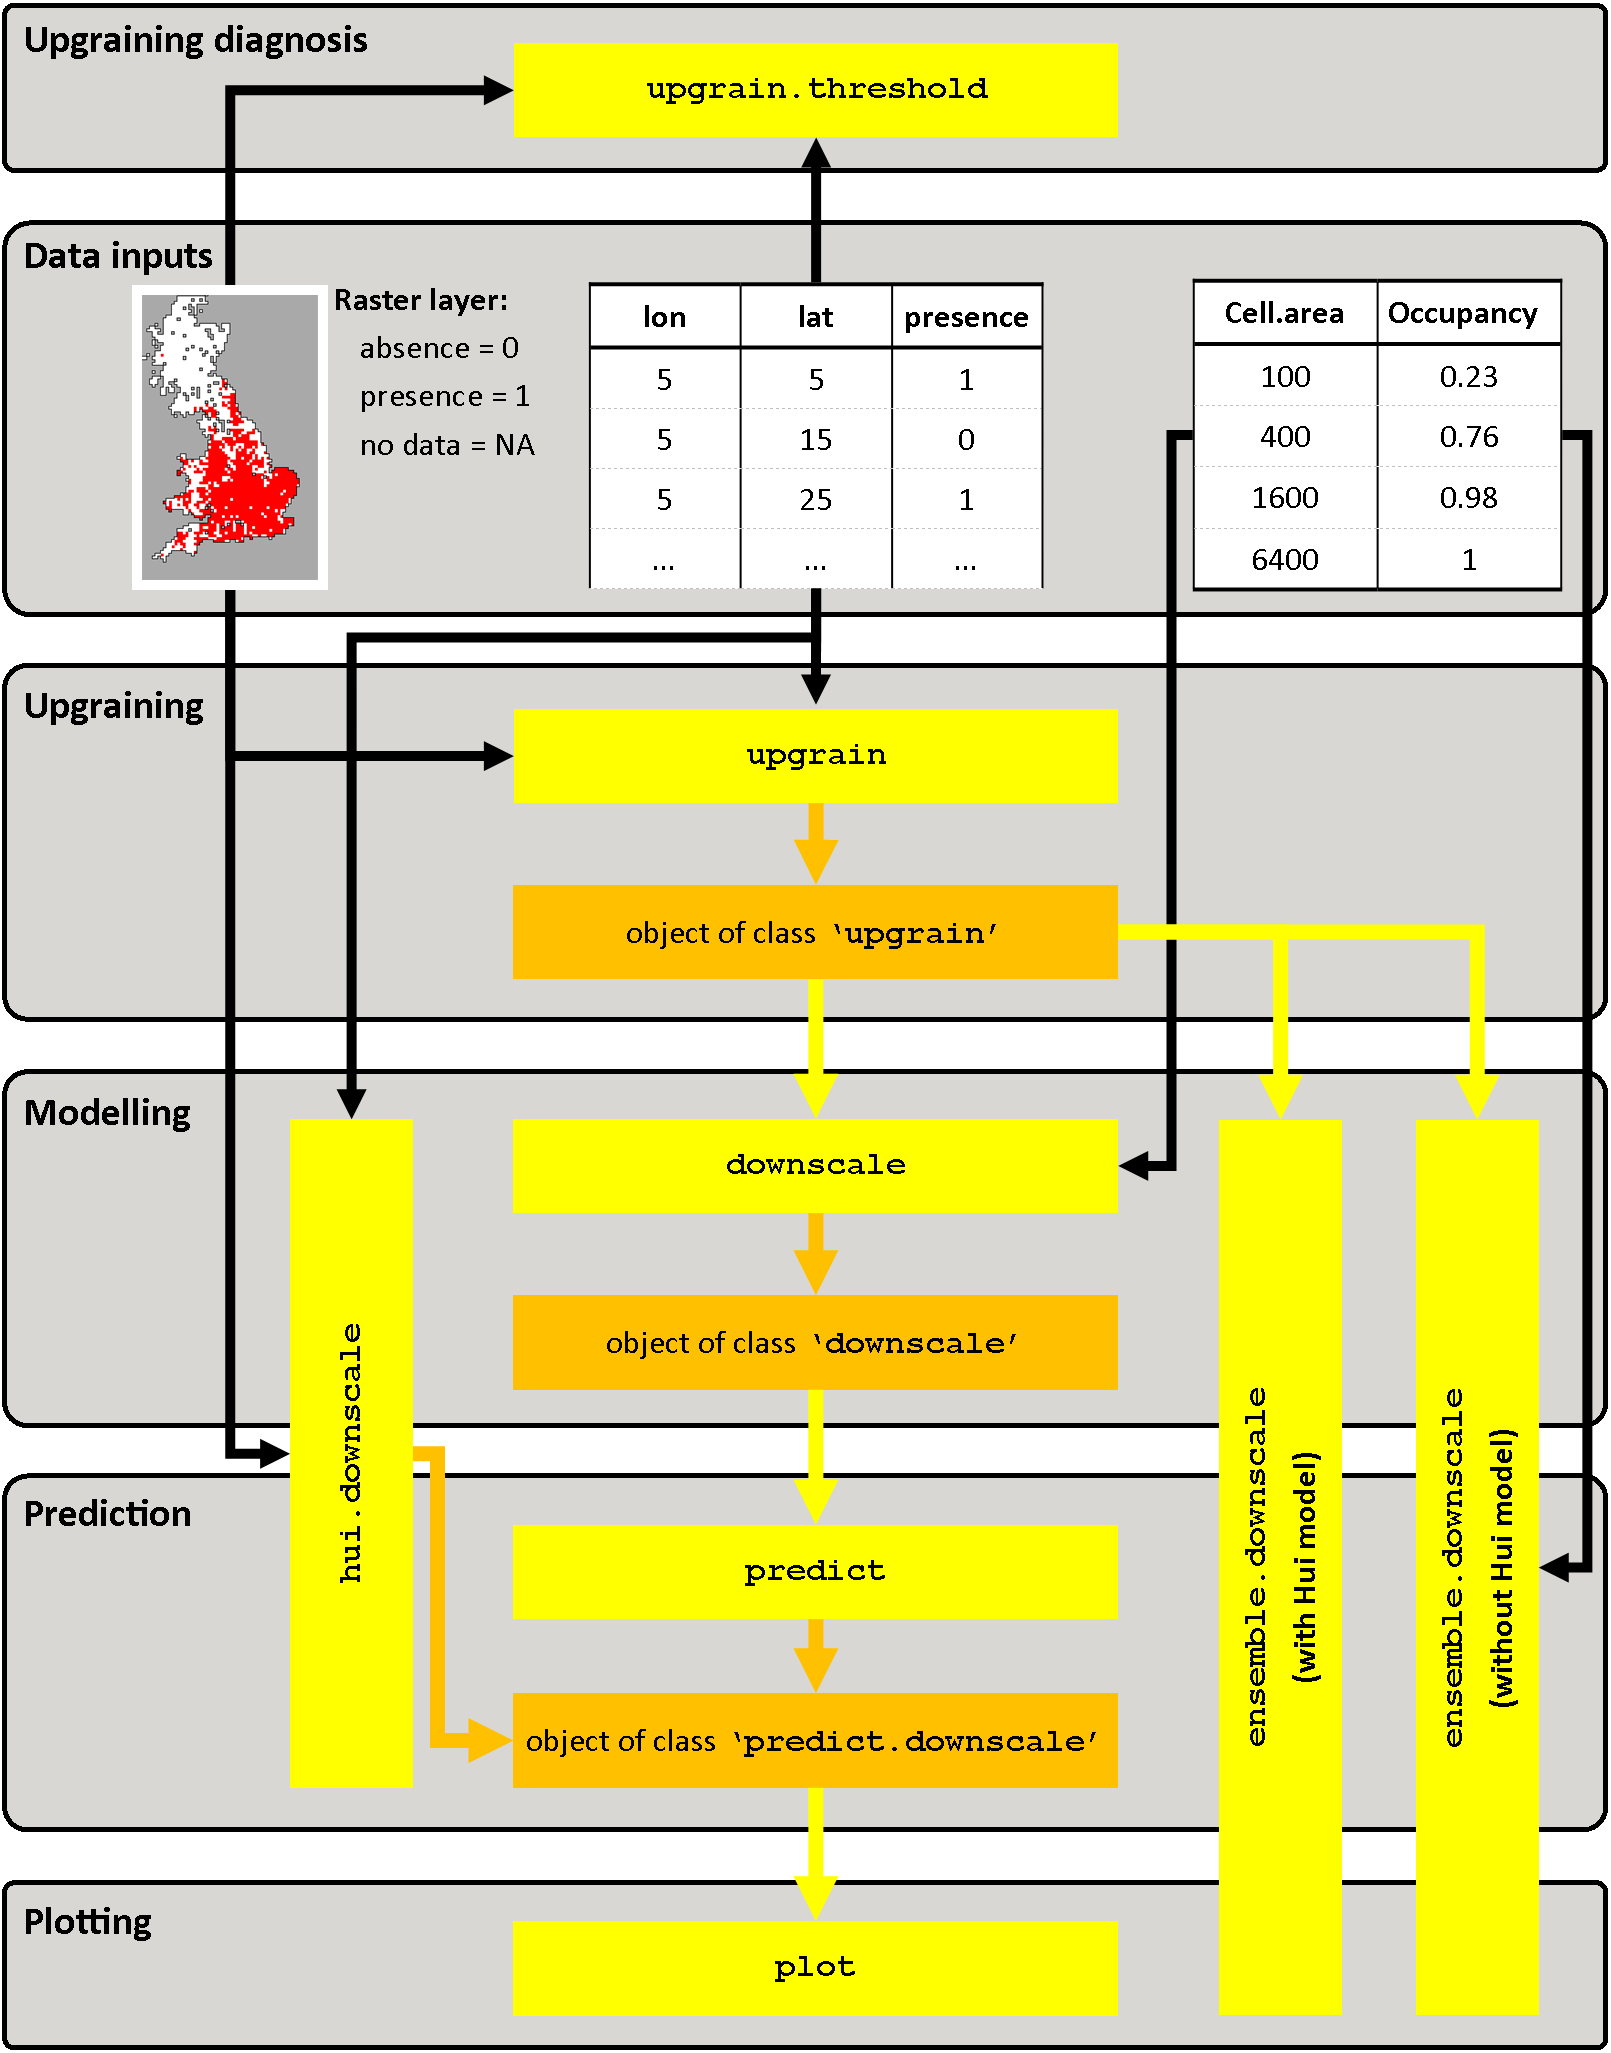
\includegraphics[width=\linewidth]{Flow.png}
\caption{Structure of the \texttt{downscale} package showing all eight functions (yellow) and the three output object classes (orange).}
\label{fig:Flow}
\end{figure}

The user may input three types of data:
\begin{enumerate} \itemsep1pt \parskip0pt 
\item [1)] A data frame of grain sizes (cell area) and occupancies in that order;
\item [2)] A data frame of sample (cell) coordinates and presence-absence data (presence = 1; absence = 0). Column names must be “lon”, “lat”, and “presence”;
\item [3)] A raster layer of presence-absence data (presence = 1; absence = 0; no data = NA).
\end{enumerate}

If the user wishes to carry out downscaling with the Hui model (Hui et al. 2006, 2009) or upgraining of atlas data (and exploration of upgraining thresholds) then the input data must be of type 2 or 3. Table 1 shows the functions to use to achieve desired objectives with regards to input data.

\begin{table}[!h]
\begin{tabular}{| p{3.9cm} | p{3.5cm} | p{4.1cm} |}
\hline
\textbf{Input data type} & \textbf{Objective} & \textbf{Function flow}  \\\hline
Data frame of cell areas and occcupancies & Downscale (excluding Hui model) & \parbox[t]{0.1cm}{ \texttt{downscale}\Rightarrow \ \texttt{predict}\Rightarrow \ \texttt{plot}}
\\\hline
Data frame of cell coordinates and presence-absence data & Downscale (excluding Hui model) & \parbox[t]{0.1cm}{ \texttt{upgrain.threshold}\Rightarrow\ \texttt{upgrain} \Rightarrow\  \texttt{downscale}\Rightarrow\ \texttt{predict}\Rightarrow\ \texttt{plot}}
\\\hline
Raster layer of presence-absence data & Downscale (excluding Hui model)	& \parbox[t]{0.1cm}{ \texttt{upgrain.threshold}\Rightarrow \ \texttt{upgrain}\Rightarrow \ \texttt{downscale}\Rightarrow \ \texttt{predict}\Rightarrow \texttt{plot}}
\\\hline
Data frame of cell coordinates and presence-absence data &	Downscale (including Hui model)	& \parbox[t]{0.1cm}{ \texttt{hui.downscale}\Rightarrow \ \texttt{plot}}
\\\hline
Raster layer of presence-absence data &	Downscale (including Hui model) &	\parbox[t]{0.1cm}{ \texttt{hui.downscale}\Rightarrow \ \texttt{plot}}
\\\hline
Data frame of cell coordinates and presence-absence data &	Ensemble modelling (excluding Hui model) &	\parbox[t]{0.1cm}{\texttt{ensemble.downscale}}
\\\hline
Raster layer of presence-absence data &	Ensemble modelling (with or without Hui model) &	\texttt{upgrain.threshold}\Rightarrow \ \texttt{upgrain}\Rightarrow \ \texttt{ensemble.downscale}}
\\\hline
\end{tabular}
\caption{Flow of functions for different objectives depending on data input type.}
\end{table}


For downscale modelling it is important they check their data for the scale of saturation and endemism. The scale of saturation is the grain size where all cells are occupied (fig. \ref{fig:Saturation}a). The scale of endemism is the grain size where the entire distribution occurs in a single cell (\ref{fig:Saturation}b). All occupancies above these grain sizes should be set to NA, as they are providing no information for the occupancy-area curve. The downscale functions will automatically set these occupancies to NA for modelling purposes, which can lead to not enough scales remaining for downscaling.

\begin{figure}[!t]
\centering
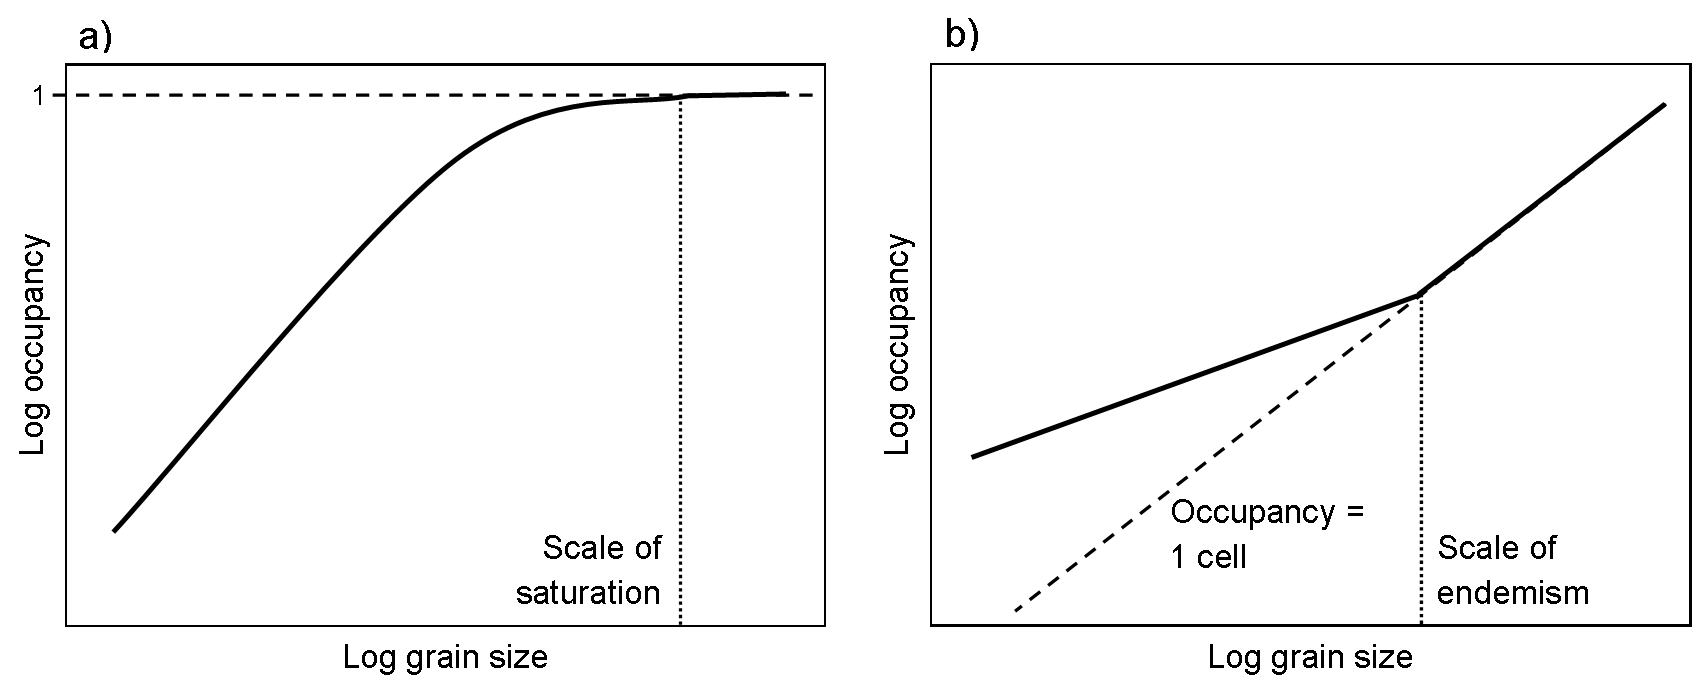
\includegraphics[width=\linewidth]{Saturation.png}
\caption{Occupancy-area relationships for two species showing a) the scale of saturation (the grain size at which all cells are occupied – ie occupancy = 1) and b) the scale of endemism (the scale at which only one cell is occupied). Occupancies of all grain sizes above these points should be set to NA.}
\label{fig:Saturation}
\end{figure}

\section{Package tutorial}

First, we must download the downscale package from R-forge.

\begin{Schunk}
\begin{Sinput}
> install.packages("downscale",
+                  repos = "http://R-Forge.R-project.org")
\end{Sinput}
\end{Schunk}

Then load in the library

\begin{Schunk}
\begin{Sinput}
> library("downscale")
\end{Sinput}
\end{Schunk}

\subsection{A quick example}
We will start with the simplest example of using the downscaling package, where we already have occupancy data across a number of spatial scales (grain size). In this tutorial, we’ll create some dummy data; a data frame where the first column are the cell areas (grain size) and the proportion of occupancy as the second column:

\begin{Schunk}
\begin{Sinput}
> occupancy <- data.frame(Cell.area = c(100, 400, 1600, 6400),
+                         Occupancy = c(0.23, 0.56, 0.87, 1))
\end{Sinput}
\end{Schunk}

Now we use downscale to estimate the model parameters for the logistic model to the data (note: for this type of data input we must also specify the total extent):

\begin{Schunk}
\begin{Sinput}
> logis.mod <- downscale(occupancies = occupancy,
+                        model = "Logis",
+                        extent = 320000)
> ## this creates an object of class ‘downscale’
> logis.mod
\end{Sinput}
\begin{Soutput}
$model
[1] "Logis"

$pars
          C           z 
0.002014927 1.083725424 

$observed
  Cell.area Occupancy
1       100      0.23
2       400      0.56
3      1600      0.87
4      6400      1.00

$extent
[1] 320000

attr(,"class")
[1] "downscale"

\end{Soutput}
\end{Schunk}

Using the modelled parameters from the \texttt{‘downscale’} object we can predict occupancies at finer grain sizes. We will first create a vector of cell sizes (area) to predict. If we include the original cell sizes used for modelling we can also observe the model fit.

\begin{Schunk}
\begin{Sinput}
> areas.pred <- c(1, 2, 5, 25, 100, 400, 1600, 6400)
> logis.pred <- predict(logis.mod,
+                       new.areas = areas.pred)
> ## this creates an object of class ‘predict.downscale’
> ## occupancy is given as a proportion and area of occupancy (AOO)
> logis.pred$predicted
\end{Sinput}
\begin{Soutput}
  Cell.area   Occupancy         AOO
1         1 0.002010876    643.4802
2         2 0.004252482   1360.7942
3         5 0.011396541   3646.8932
4        25 0.061873397  19799.4871
5       100 0.228564935  73140.7793
6       400 0.570999511 182719.8435
7      1600 0.856717834 274149.7068
8      6400 0.964106833 308514.1867

\end{Soutput}
\end{Schunk}
\begin{Schunk}
\begin{Sinput}
> ## now we can plot the predictions
> plot(logis.pred)
\end{Sinput}
\end{Schunk}
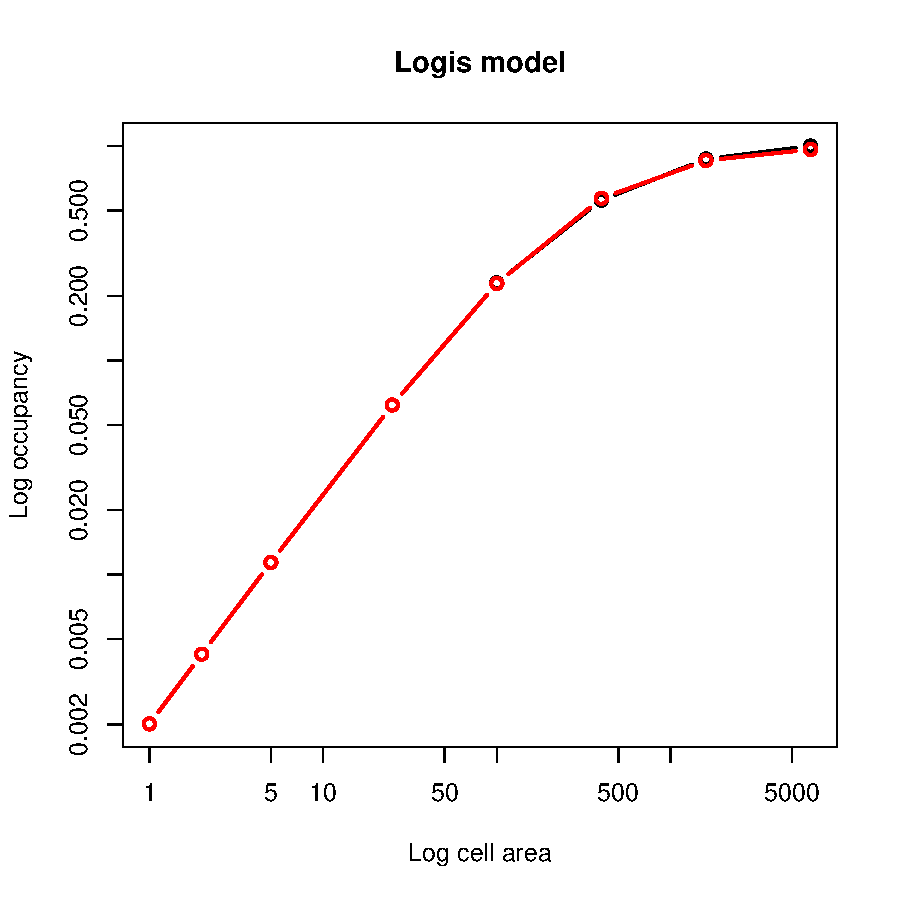
\includegraphics{Downscaling-downscale6}

\subsection{Using atlas data}
For the majority of cases we will only have atlas data that first needs to be upgrained. Read in example atlas data for the UK (in this case a data frame of sample cell coordinates and presence-absence data):

\begin{Schunk}
\begin{Sinput}
> ## if it is not already loaded, load in the package
> library(downscale)
> data.file <- system.file("extdata", "atlas_data.txt", package = "downscale")
> atlas.data <- read.table(data.file, header = TRUE)
\end{Sinput}
\end{Schunk}

The data frame must have the column names “lon”, “lat” and “presence”:

\begin{Schunk}
\begin{Sinput}
> head(atlas.data)
\end{Sinput}
\begin{Soutput}
   lon lat presence
1 8170  10        0
2 8130  20        0
3 8140  20        0
4 8160  20        0
5 8170  20        0
6 8140  30        0

\end{Soutput}
\end{Schunk}

The first step is to upgrain the atlas data to calculate occupancy at larger grain sizes than the atlas data – this provides the proportion of occupancy data points to fit the different downscaling models to. Therefore it is important that we fix the extent for all grain sizes, but this means compromising between assigning unsampled cells as absences or excluding sampled cells as No Data. We can explore this trade-off with \texttt{upgrain.threshold}:

\begin{Schunk}
\begin{Sinput}
> ## explore thresholds using upgrain.threshold
> thresh <- upgrain.threshold(atlas.data = atlas.data,
+                             cell.width = 10,
+                             scales = 3,
+                             thresholds = seq(0, 1, 0.01))